\begin{figure}
    \centering
        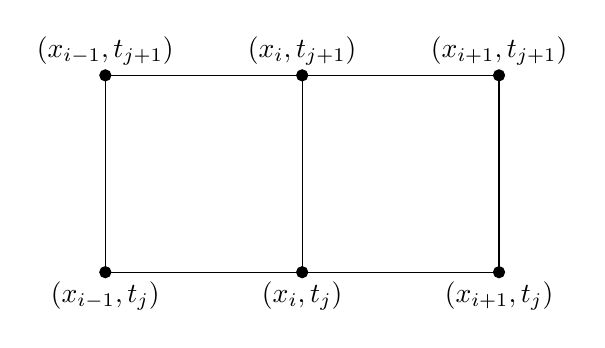
\begin{tikzpicture}
            \draw (-2.5, 0) -- (2.5, 0);
            \draw (-2.5, 2.5) -- (2.5, 2.5);
            \draw (-2.5, 0) -- (-2.5, 2.5);
            \draw (0, 0) -- (0, 2.5);
            \draw (2.5, 0) -- (2.5, 2.5);

            \filldraw[black] (-2.5, 0) circle(2pt) node[anchor=north] {$(x_{i - 1}, t_{j})$};
            \filldraw[black] (0, 0) circle(2pt) node[anchor=north] {$(x_{i}, t_{j})$};
            \filldraw[black] (2.5, 0) circle(2pt) node[anchor=north] {$(x_{i + 1}, t_{j})$};
            \filldraw[black] (-2.5, 2.5) circle(2pt) node[anchor=south] {$(x_{i - 1}, t_{j + 1})$};
            \filldraw[black] (0, 2.5) circle(2pt) node[anchor=south] {$(x_{i}, t_{j + 1})$};
            \filldraw[black] (2.5, 2.5) circle(2pt) node[anchor=south] {$(x_{i + 1}, t_{j + 1})$};
            
            % \draw (-2.5, 0) node[anchor=north] {$(x_{i - 1}, t_j)$} -- (2.5, 0) node[anchor=north] {$(x_{i + 1}, t_j)$};
            % \draw (-2.5, 2.5) node[anchor=north] {$(x_{i - 1}, t_{j + 1})$} -- (2.5, 2.5) node[anchor=north] {$(x_{i + 1}, t_{j + 1})$};
            % \draw (0, 0) -- (0, 2.5) node[anchor=south]{$(x_i, t_{j + 1})$};
            % \filldraw[black] (0, 0) circle(2pt) node[anchor=south west] {$(x_i, t_j)$};
            % \filldraw[black] (-2.5, 0) circle(2pt);
            % \filldraw[black] (2.5, 0) circle(2pt);
            % \filldraw[black] (0, 2.5) circle(2pt);
        \end{tikzpicture}
    \caption{Шеститочечный шаблон явной схемы}
    \label{fig:implicit_template}
\end{figure}
Идея неявных схем заключается в использовании шаблона, затрагивающего как значения функции на $j$--ом временном слое (который предполагается уже известным), так и на последующих слоях (значения функции на которых ещё не известны).
Так, однопараметрическое семейство неявных схем, зависящих от параметра $\sigma \in (0, 1]$ получается при аппроксимации дифференциального оператор на шеститочечном шаблоне (\seefigref{fig:implicit_template}), причём значения на \glqq верхнем\grqq и \glqq нижнем\grqq временных слоях берутся с весами $\sigma$ и $1 - \sigma$ соответственно.
Так, аппроксимация дифференциального оператора для одномерного уравнения с постоянными коэффициентами выглядит следующим образом:
\begin{multline*}
    L = \frac{\partial u}{\partial t} - \Delta u \mapsto 
    L_{h\tau} =\\
    = \frac{u_i^{j + 1} - u_i^j}{\tau} -
    \sigma\frac{u_{i + 1}^{j + 1} - 2u_i^{j + 1} + u_i^{j + 1}}{h^2}  -
    (1 - \sigma)\frac{u_{i + 1}^j - 2u_i^j + u_i^j}{h^2} + \phi_i^j,\\
    \phi_i^{j + 1} = f(x_i, t_{j + 1})
\end{multline*}
В многомерном случае можно задавать целый вектор $\sigma = (\sigma_1 \ldots \sigma_n)$:
\begin{multline*}
    L \mapsto 
    \frac{u_i^{j + 1} - u_i^j}{\tau} + \\
    + \sum\limits_{k = 1}^{n} \left[ 
        \sigma_k\frac{u_{i+}^{j + 1} - 2u_i^{j + 1} + u_{i-}^{j + 1}}{h_k^2} +
        (1 - \sigma_k) \frac{u_{i+}^j - 2u_i^j + u_{i-}^j}{h_k^2}
    \right] +\\
    + \phi_i^j,\text{ где }\\
    i_{\pm} = (i_1, \ldots, i_{k - 1}, i_k \pm 1, i_{k + 1}, \ldots, i_n)
\end{multline*}
Аналогично явной схеме, добавляя граничные и начальные условия, получаем замкнутую систему линейных уравнений.
Однако, в отличие от явной схемы, значения на новом временном слое $u^{j + 1}$ не выражаются явно через значения на предыдущем временном слое $u^{j}$, а получаются путём решения соответствующей системы линейных алгебраических уравнений $M u^{j + 1} = D$.
В одномерном случае матрица системы получается \emph{трёхдиагональной}:
\begin{equation*}
    M = \begin{pmatrix}
        B_1 & C_1 & 0 & 0 & 0 & 0 & 0\\
        A_2 & B_2 & C_2 & 0 & 0 & 0 & 0\\
        0 & A_3 & B_3 & C_3 & 0 & 0 & 0\\
        0 & 0 & A_4 & B_4 & C_4 & 0 & 0\\
        0 & 0 & 0 & \ddots & \ddots & \ddots & 0\\
        0 & 0 & 0 & 0 & A_{n-1} & B_{n-1} & C_{n-1}\\
        0 & 0 & 0 & 0 & 0 & A_{n} & B_{n}
    \end{pmatrix},
\end{equation*}
где 
\begin{align*}
    & A_i = -\sigma \tau\\
    & B_i = h^2 + 2\sigma \tau\\
    & C_i = -\sigma \tau\\
    & D_i = h^2 u_i^j + \tau (1 - \sigma) \left( 
        u_{i - 1}^j - 2u_i^j + u_{i + 1}^j
     \right) + \tau h^2 \phi_i^{j + 1}
\end{align*}
В таком случае существует эффективный алгоритм расчёта, именуемый \emph{методом прогонки}:
Сначала определяем $\alpha$ и $\beta$:
$$
    \begin{cases}
        \alpha_1 = -\frac{C_1}{B_1}, \\
        \beta_1 = \frac{D_1}{B_1}, \\
        \begin{aligned}
            & \alpha_i = -\frac{C_i}{B_i + A_i \cdot \alpha_{i-1}}\\
            & \beta_i = \frac{D_i - A_i \cdot \beta_{i-1}}{B_i + A_i \cdot \alpha_{i-1}}
        \end{aligned}, & i = 2, \ldots, n-1\\
        \beta_n = \frac{D_n - A_n \cdot \beta_{n-1}}{B_n + A_n \cdot \alpha_{n-1}}
    \end{cases}
$$
Затем по ним определяем неизвестные:
$$
    \begin{cases}
        x_n = \beta_n,\\
        x_i = \alpha_i \cdot x_{i+1} + \beta_i, & i = n-1, \ldots, 1
    \end{cases}
$$
Сложность такого алгоритма $O(N_x)$, что не уступает явной схеме.
Преимущества же неявной схемы в том, что для неё условия устойчивости принимает вид
\begin{equation*}
    \sigma \geqslant \frac{1}{2} - \frac{h^2}{4\tau}.
\end{equation*}
Из этого условия видно, что при $\sigma \ge 0.5$ схема безусловно устойчива, то есть устойчива вне зависимости от выбора шагов $h$ и $\tau$.

При значениях $\sigma \ne 0.5$ схема имеет порядок точности $O(h^2 + \tau)$, а при $\sigma = 0.5$ (так называемая \emph{схема Кранка-Николсона}) $O(h^2 + \tau^2)$, то есть больший, явная схема.

Недостатком такой схемы является отсутствие возможности распараллеливания.

В случае многомерной задачи дело обстоит хуже.
Получаемые системы линейных уравнений имеют более сложную матрицу (не трёхдиагональную). Для их решения пользуются в общем случае методом последовательного исключения переменных (методом Гаусса), который работает за $O(N^3)$, где $N \times N$~--- размерность матрицы.
Так, уже в двумерной задаче матрица будет размера $N_xN_y \times N_x N_y$, и расчёт будет проводиться заметно дольше, чем при расчёте явной схемой ($\sim O(N^2)$).